\chapter{Computing Fundamentals in LabVIEW}
In this chapter, we will go over some of the basic building blocks of a computer program in the context of $\labview$. This chapter will be heavy on examples in $\labview$, but will be light on the trivial details such as how to open a VI and how to place functions and controls. If you have not already done so, review the exercise in section \ref{HowToPlace} in Chapter 1.\\

If you get stuck, you may open the $\labview$ help files my pressing \texttt{Ctrl+?} and navigating to the ``Fundamentals'' section. If you would like to see more examples of how things are done in $\labview$, on the taskbar select ``Help'' and navigate down the menu to find ``Find Examples...'', here you will find a library of examples. These examples range from trivial arithmetic, to programs which would make you a cup of coffee if you supply it with enough hardware.

\section{Decision making structures}
Without the ability to make decisions, computers would not be as useful as they are now. Try to think of a computer program that makes no decisions based on it's input, they do exist and some are even useful. We are not interested in such academic programs, we want our computer to do the heavy lifting for us, just imagine clicking \texttt{yes} or \texttt{no} for a data set of a billion numbers. My computer can do that in $5.76$ seconds (I just checked using $\labview$).\\

If you are familiar with programming, you know that the most fundamental decision making block is an ``if-statement''. You supply the block with a condition, and the program executes statements based on that condition. Technically speaking, $\labview$ has no such thing as an if-statement, it has ``case-structures'' and ``ternary-operators''.

\subsection{Case Structures}
The case structure executes a block of code according to its input condition. In $\labview$, the input condition may be either a boolean value, an enumeration, or an error value. Figure \ref{ch2egTrue} (A) shows how a case structure looks, a thick grey box with a green \texttt{?} and a selection box stating ``True''. What ever is inside this grey box will be executed if a boolean true value is wired into the conditional terminal, the green \texttt{?}. Figure \ref{ch2egFalse} shows what would be executed if the condition is false.\\
\begin{figure}
	\centering
	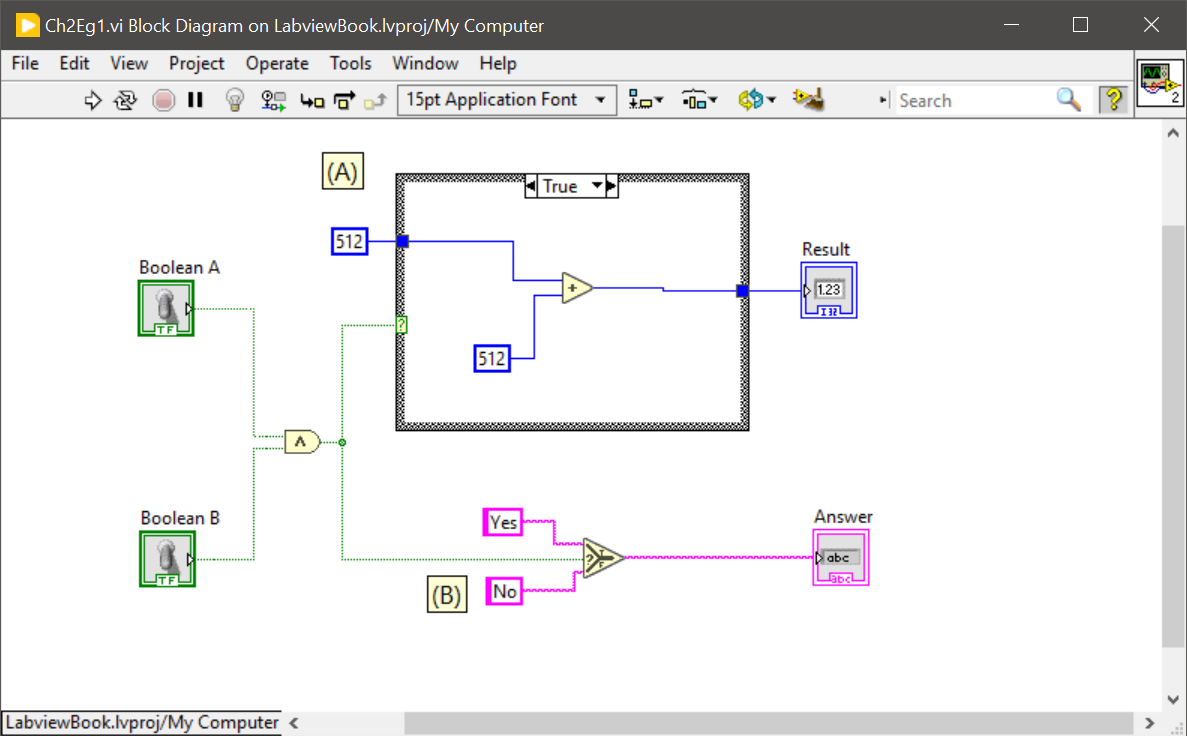
\includegraphics[width=\textwidth]{ch2eg1True}
	\caption{A case structure showing its truth block (A), and a ternary operator (B).}
	\label{ch2egTrue}
\end{figure}
\begin{figure}
	\centering
	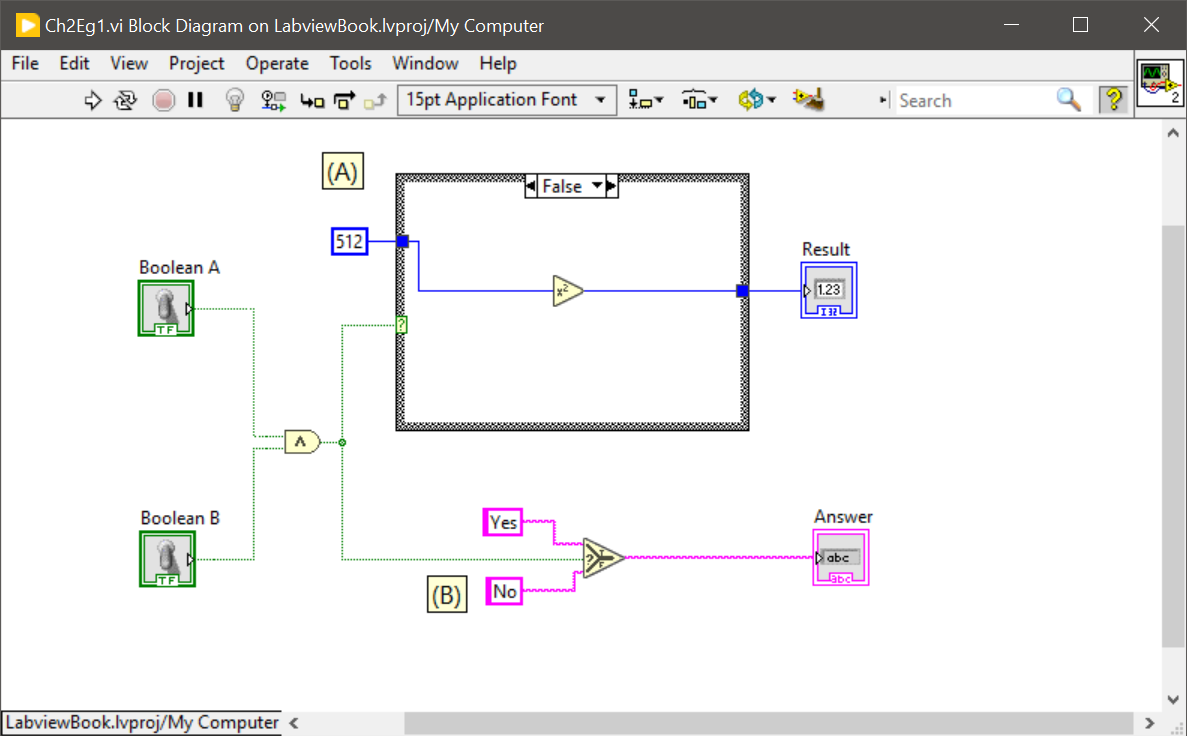
\includegraphics[width=\textwidth]{ch2eg1False}
\caption{A case structure showing its false block (A), and a ternary operator (B).}
\label{ch2egFalse}
\end{figure}

Comparison functions in $\labview$ produce only boolean values, this you have seen in the examples so far. Feeding these boolean values into case structures allow you to select different operations to be preformed. The example provided in figures \ref{ch2egTrue} \& \ref{ch2egFalse} show how you would choose two different operations on an integer. If the condition is true, 512 is added to the input number and the result is given, the indicator outside the case structure.  If the value is false, 512 is squared and the result given.\\

A case structure also accepts enumeration values. This is similar to a switch structure in \texttt{C} programming. In figure \ref{ch2eg2}, a value named ``Multiply'' is placed into the case structure. This allows you to have many paths of execution in a single structure. In the example, a simple calculator is made which takes two input numbers and an enumeration condition, the block then executes the proper logic and hands you the result at the end. One of the mini projects at the end of this chapter will require you to create a 4-function calculator.\\
\begin{figure}
	\centering
	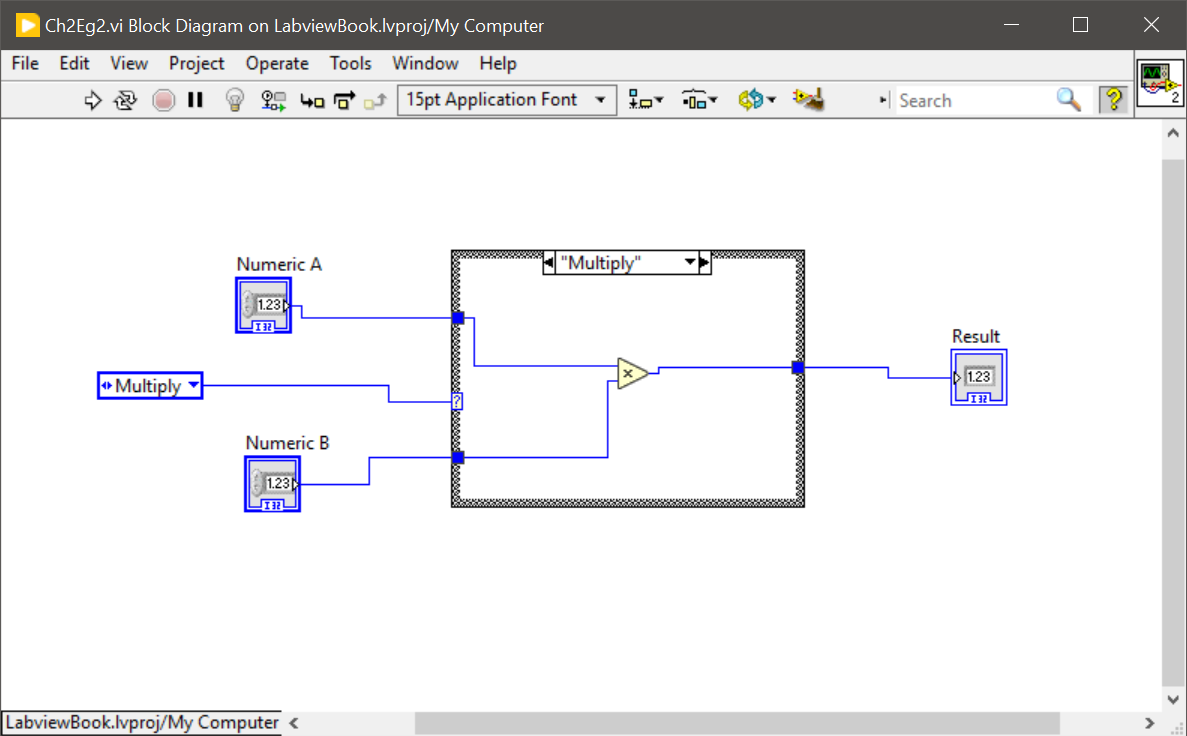
\includegraphics[width=\textwidth]{ch2eg2}
\caption{A simple calculator using an enumeration type and a case structure.}
\label{ch2eg2}
\end{figure}

\subsection{Ternary operators}
The plural in the title is misleading, there is only one ternary operator in $\labview$. Figure \ref{ch2egTrue} (B), on page \pageref{ch2egTrue}, is this little function in action. You supply it with a boolean value and outputs either its truth or false value. In this example, if the boolean value is true, then the ternary operator outputs the string ``Yes''.\\

The only caveat is that you must use the same variable type for its true and false inputs, this type will also be its output type.  There really isn't anything more special about the ternary operator. It is possible to implement a ternary operator using a case structure, an exercise left for the reader.

\section{Code looping structures}
In the previous section, I mentioned that my computer could make a billion decisions in $5.76$ seconds. The program certainly did not contain a billion case structures, it only had one.\\

It is quite rare for a program to only make one decision before execution stops, most probably you have a few decisions which would need to be repeated thousands of times per execution. One may even say that you would like to have a program perform a ``loop'' of decisions. This is were loop structures come into play.\\

The two loop structures available to us in $\labview$ is the ``For Loop'' and the ``While Loop''. The for loop executes a set number of times while the while loop executes until some specified condition is met. These two structures are closely related however since the for loop can pretend to be a while loop. It is also worth mentioning in passing, to those of you with previous programming experience, that both loops act as `do-while'' loops since they execute at least once before evaluating their conditional terminals.\\

The flow of information in $\labview$ is rather unconventional, this will be elaborated upon in a future section, but for now there will be references to arrays, time functions, and shift registers without going into depth for either topics.

\subsection{For Loops}
A for loop executes a predetermined amount of times. Figure \ref{ch2eg3} is perhaps the most simple, yet interesting, loop possible in $\labview$. You set the number of times the loop should run in the ``Number of times'' control and the loop shows you the iteration step number along with a random floating point number between 0 \& 1. The little watch function in the bottom right corner is to slow the loop execution speed to twice every second so you are able to observe the number generated.\\
\begin{figure}
	\centering
	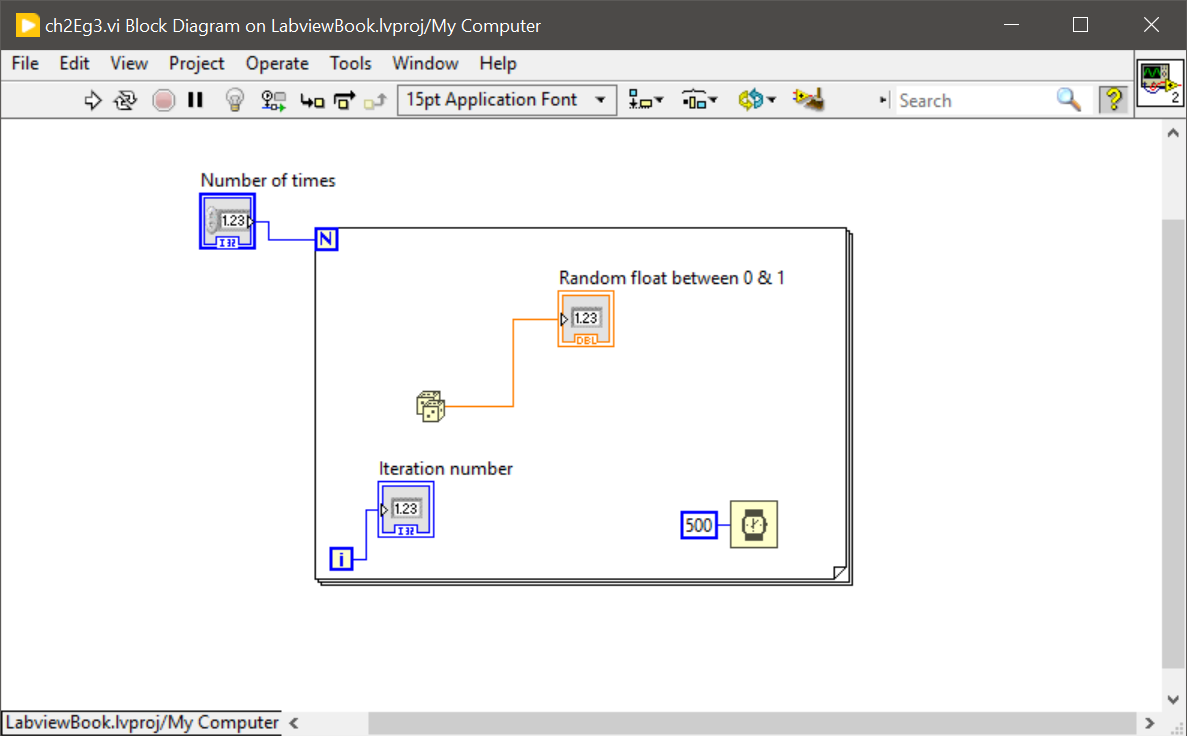
\includegraphics[width=\textwidth]{ch2eg3}
	\caption{A simple loop that ejects random numbers, two every second.}
	\label{ch2eg3}
\end{figure}

The example is heavily constrained however, there is no way for the information generated to be stored in memory so there is no knowlage for what the random number was in the previous iteration let alone what the series of generated numbers were.\\

Just by introducing a concept known as a shift register, we can actually start making useful programs, or what ever useful means in this case. A shift register allows you to store a variable from a current loop iteration so that it is useable in the next iteration. To illustrate this, let us create a loop that prints out, in sequence, the first 10 numbers in the Fibonacci sequence.\\

The Fibonacci sequence, defined by the recurrence relation:
\begin{equation*}
	F_0=0,\quad F_1=1,\quad F_n= F_{n-1} + F_{n-2}
\end{equation*}
An implementation of this may be found in figure \ref{ch2eg4}. On the right hand side of the loop structure is a little blue arrow in a box, this is the terminal where you value the number you want available to the next loop iteration. To add a shift register to a loop, \texttt{right click} on any side of the loop frame and select ``Add Shift Register'' from the drop-down menu.\\
\begin{figure}
	\centering
	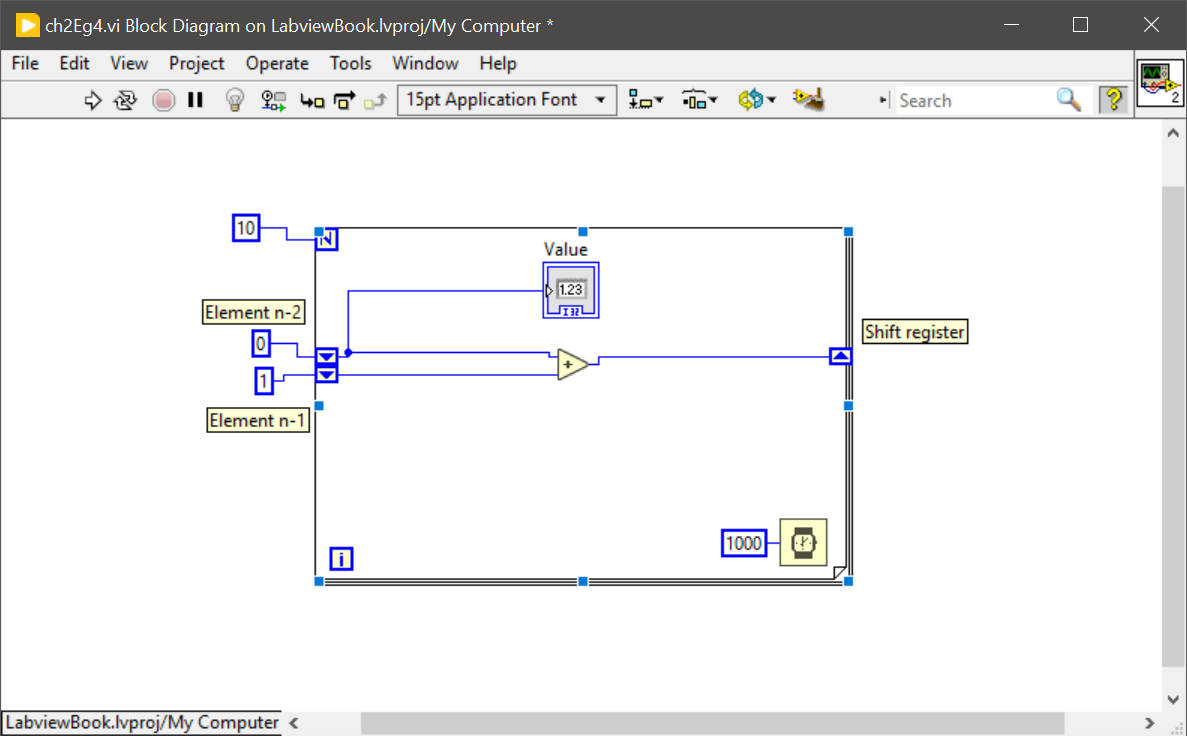
\includegraphics[width=\textwidth]{ch2eg4}
	\caption{A loop that displays the Fibonacci numbers, updating every second.}
	\label{ch2eg4}
\end{figure}

You may notice in that example that the left hand side has two little arrows stacked on top of each other, this gives you access to the previous iteration values. In this case the top arrow is the value of iteration n-2 and the bottom arrow is the value of iteration n-1. You can extend or reduce the number of iterations available by clicking and dragging the bottom edges of the shift register.\\

The values feeding into the left of the shift registers initialise the two first numbers in the sequence. If you do not do this, the two initial numbers would be $0$. Do not rely on such implicit details, if you want to have the first numbers to be $0$, wire in a zero constant explicitly. This will also show your intent in the code and not leave people reading the code guessing.\\

The indicator wired to the little blue \texttt{i} gives you access to the current iteration, starting from $0$ end ending in $n-1$. You don't need to memorise this, just hover your mouse over the little blue \texttt{i} and it will tell you. Although not exactly useful in this example, it makes working with arrays significantly easier so you should look forward to that.\\

\subsection{While Loops}
Suppose your program needs to monitor a temperature sensor and it requires the temperature to be above some set point before it turns on a fan, say. You can not know when this temperature threshold is reached, if it is ever ever reached. In such a case, a while loop allows us to execute some code only leaving the loop once some condition is met. If the condition is never met, then the loop never ends.\\

Figure \ref{ch2eg5} is the previous Fibonacci sequence program modified to use a while loop instead. Gone is the little blue \texttt{N} in the top left corner of the loop. Instead, a little red octagon is present at the bottom right corner of the loop. This is the conditional terminal\\
\begin{figure}
	\centering
	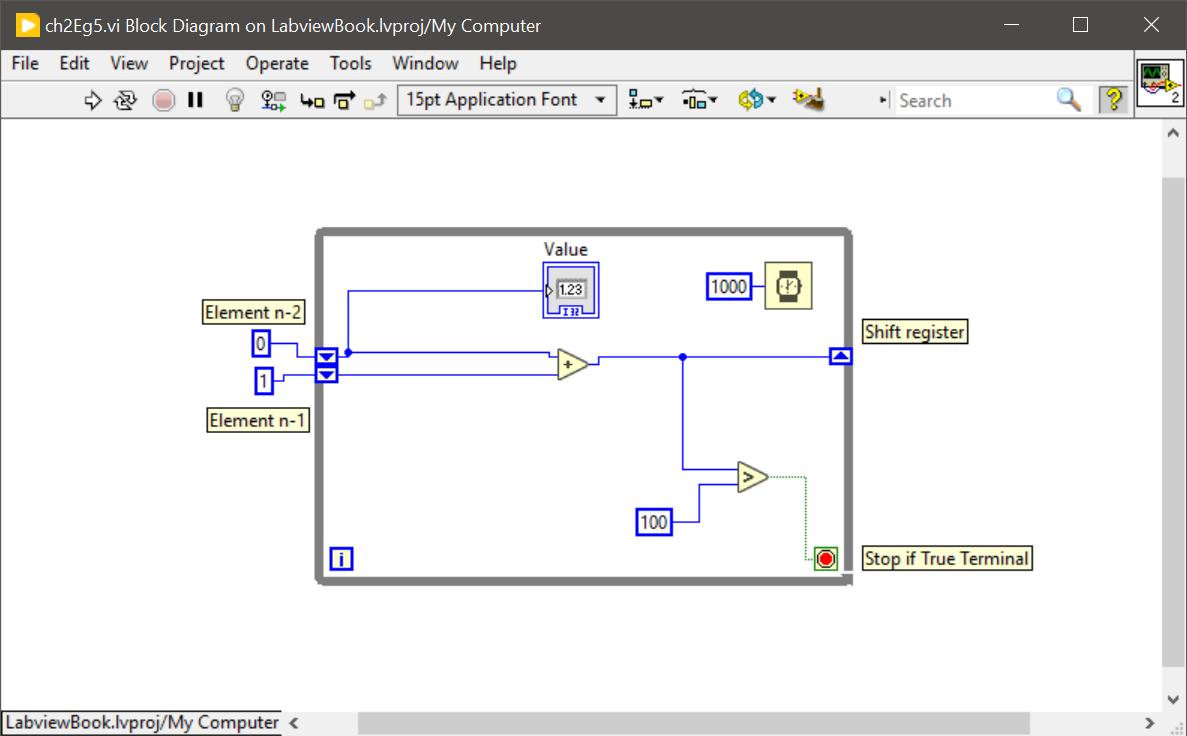
\includegraphics[width=\textwidth]{ch2eg5}
	\caption{A loop that displays the Fibonacci numbers less than 100, updating every second.}
	\label{ch2eg5}
\end{figure}

In this example, if a number in the sequence is greater than $100$, the comparison function sends a ``true'' value to the condition terminal which causes the loop to terminate. If this is slightly confusing, just remember ``Red means stop!.\\

If you \texttt{right click} on the condition terminal, you may change it to a ``Continue if true'' condition. In this case, the while loop will only terminate when it receives a ``false'' value. Conveniently, the terminal changes to a green circular arrow, in other words ``Green means go!. Figure \ref{whileCond} shows the two available condition types side by side. Yes that is a little octagon stop sign, it took me almost 5 years to notice that.\\
\begin{figure} %TODO Fix the condition figures to be the same size
	\centering
	\begin{subfigure}[b]{0.40\textwidth}
		\centering
		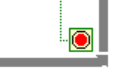
\includegraphics[width=\textwidth]{stopIfTrue}
		\caption{The ``stop if true'' while loop condition terminal.}
	\end{subfigure}
	\hfil
	\begin{subfigure}[b]{0.40\textwidth}
		\centering
		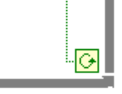
\includegraphics[width=\textwidth]{contIfTrue}
		\caption{The ``continue if true'' while loop condition terminal}
	\end{subfigure}
	\caption{The two available while loop conditions, also notice how the edge of the frame makes a little arrow.}
	\label{whileCond}
\end{figure}

Much like in other programming languages, infinite loops are considered unwanted behaviour. While loops must have their conditional terminals wired, even if your program would run for days or weeks on end, it should have a button to safely exit its execution. This will become more apparent in Chapter 3 where we will be programming hardware, other than your computer that is.\\

\section{Aggregate data types}
From here on out, the training wheels are off. The concept of an array is simple, the explanation in section \ref{ch1Arrays} is as detailed as needed and will not be repeated here. Working with arrays in $\labview$ is tricky however, in the next few pages we will dissect this creature and reveal some of the more ugly sides to this programming language.\\

\subsection{Arrays}
\subsubsection{Creation}
Technically an array is also a type of structure in $\labview$. In the block diagram view, a placed array constant contains nothing, not even a type. You provide the type by placing a constant inside the array box. This is seen preformed in figure \ref{createNumArrayConst}. In this particular case, an integer constant creates an empty integer array, seen in figure \ref{numArrayConst}.\\
\begin{figure} %TODO Fix the condition figures to be the same size
	\centering
	\begin{subfigure}[b]{0.40\textwidth}
		\centering
		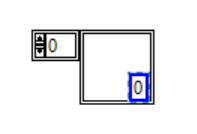
\includegraphics[width=\textwidth]{createNumArrayConst}
		\caption{An empty array constant, the integer constant has not been placed yet.}
		\label{createNumArrayConst}
	\end{subfigure}
	\hfil
	\begin{subfigure}[b]{0.40\textwidth}
		\centering
		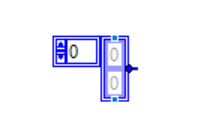
\includegraphics[width=\textwidth]{numArrayConst}
		\caption{An empty integer array constant, expanded to show two elements.}
		\label{numArrayConst}
	\end{subfigure}
	\caption{Creating an array constant.}
	\label{arrayConsts}
\end{figure}

The two little blue terminals in figure \ref{numArrayConst} are drag points to change the amount of visible elements in the array. Even if only one element is shown, you may cycle through the array using the arrows next to the $0$ seen in the figures. This $0$ corresponds to the index of the top visible element in the array. Array controls are made in a similar fashion on the front panel. Once you have made an array, you can start adding values. You do this by clicking on the grey $0$ and typing in a number.  

\subsubsection{Manipulation}
Figure \ref{ch2SimpleArrayBlock} shows how the numeric functions may be used to operate on arrays. These operations are preformed on an element by element basis. Figure \ref{ch2SimpleArrayFront} shows the result of these two operations. The result is truncated to the size of the smallest array.\\
\begin{figure}
	\centering
	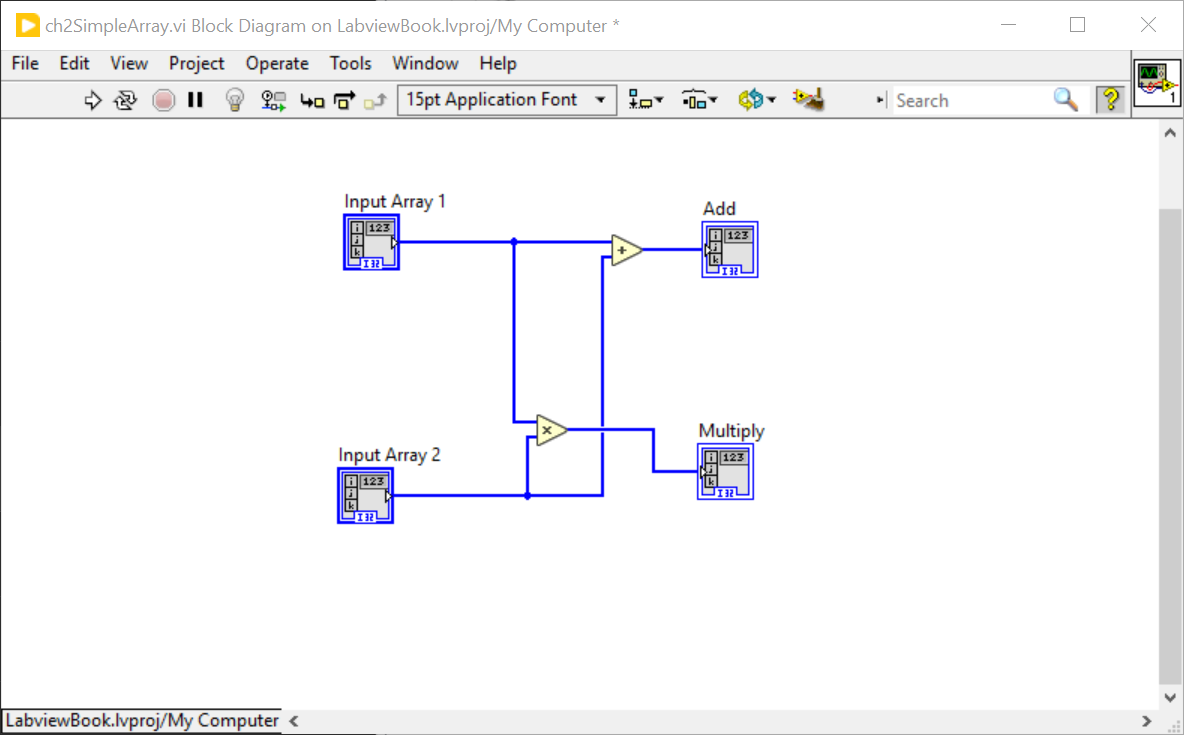
\includegraphics[width=\textwidth]{ch2SimpleArrayBlock}
	\caption{Two operations on array variables, these are the normal functions found in the ``Numeric'' folder in the functions palette.}
	\label{ch2SimpleArrayBlock}
\end{figure}
\begin{figure}
	\centering
	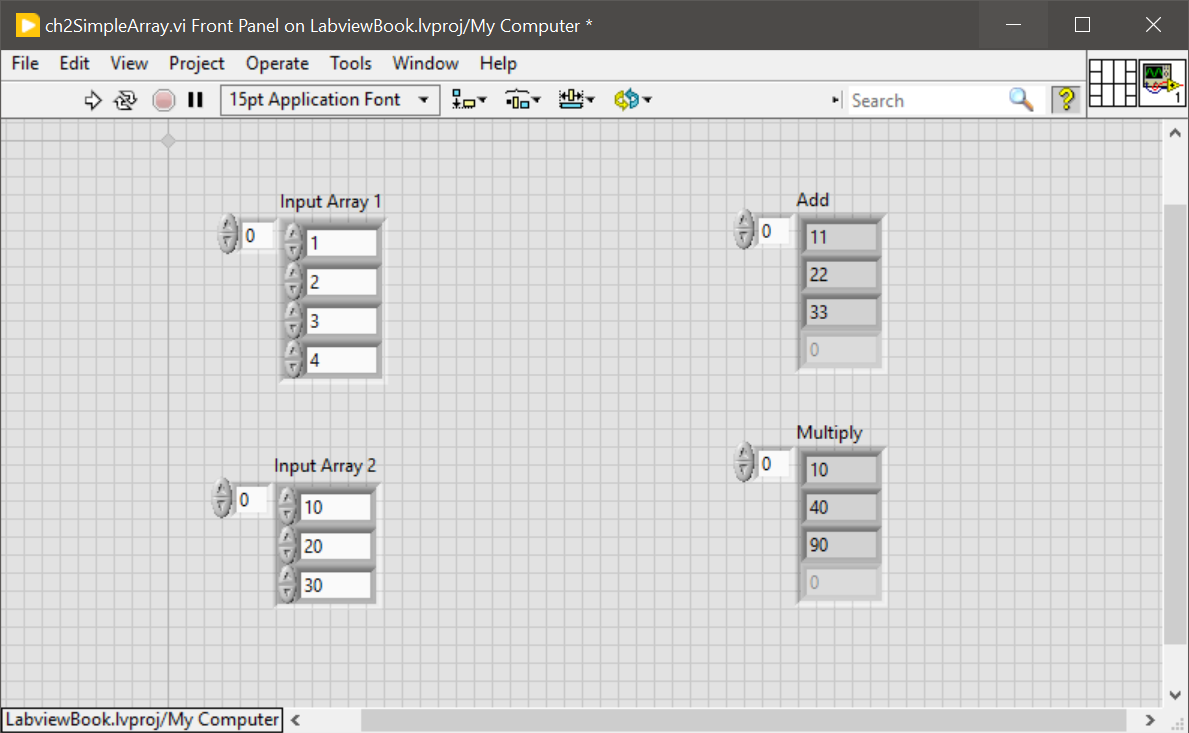
\includegraphics[width=\textwidth]{ch2SimpleArrayFront}
	\caption{The results of elementary operations on arrays.}
	\label{ch2SimpleArrayFront}
\end{figure}

There are also a few array specific functions in the numeric palette which yield the sum of all the array elements or the product all the elements. You should experiment with these on your own.\\

\subsubsection{Exploitation}
The real power, and complexity, of arrays emerge when operating on the elements themselves. Figure \ref{ch2IndexArrayBlock} shows some of the most important operations able to be performed on arrays.\\
\begin{figure}
	\centering
	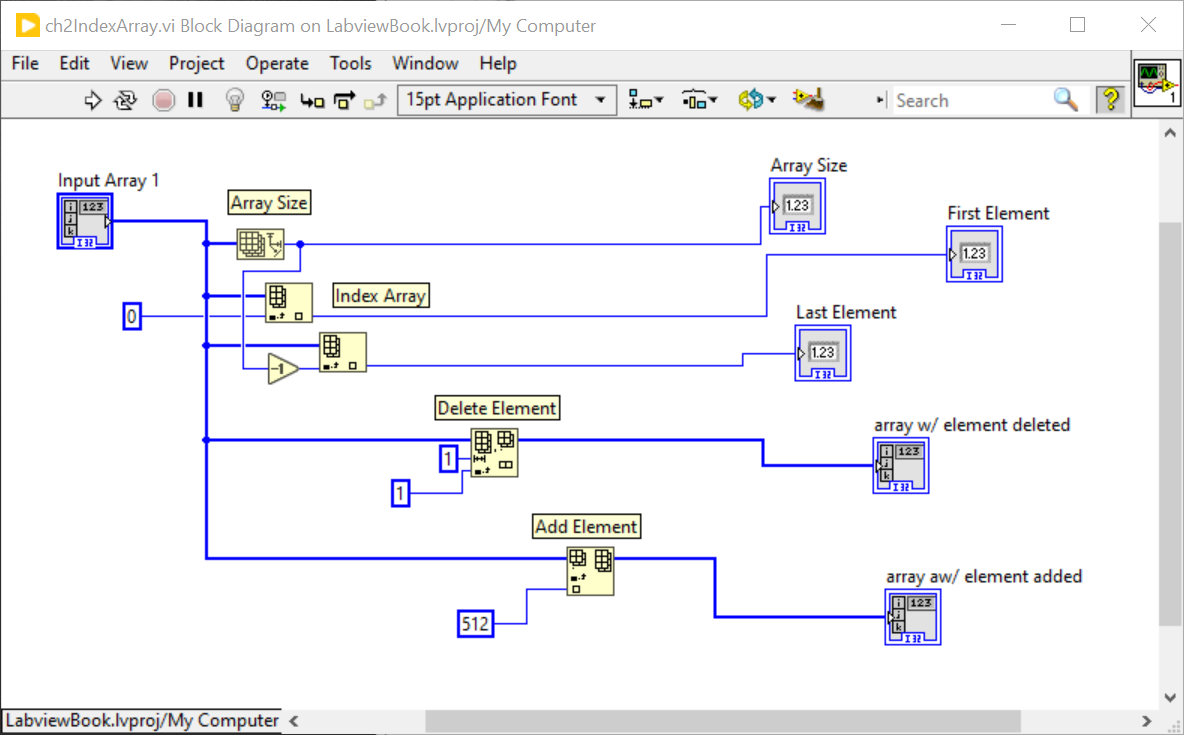
\includegraphics[width=\textwidth]{ch2IndexArrayBlock}
	\caption{Fundamental operations on arrays.}
	\label{ch2IndexArrayBlock}
\end{figure}

The array size function is rather self explanatory, it just gives you the number of elements in the array.\\

The index array function picks out an element of an array at the index you specified. Index $0$ being the first element in an array. Getting the last element of an array requires you to know its size, since indexing starts at $0$, you need to decrement the size before sending it to the index function.\\

Unlike in \texttt{C} programming, indexing an array out of bounds in $\labview$ will not destroy your computer. For numeric arrays, the index function will return $0$ upon indexing an out of range value and will continue with your program as if nothing has happened. Soon enough you will discover on your own what an ``off by one'' error is.\\

The delete array element function takes two arguments, an index value and length. This deletes the value at the selected index. If the length is more than one, the selected index and subsequent indexes are deleted. What do you think happens when you wire in a negative length value? Sadly nothing, no element is deleted if a number less than $1$ is given.\\

The add array element function adds an element into the index you specify, think of it like cutting in line at the bank. If you cut in line at position three from the front desk, the person behind you is now fourth and you are now third. I do not condone this behaviour, please exercise this in a computer program and not in real life.\\

Figure \ref{ch2IndexArrayFront} shows the results of these operations. The next step is to put these functions into context so you can see how they are used in more useful programs.\\
\begin{figure}
	\centering
	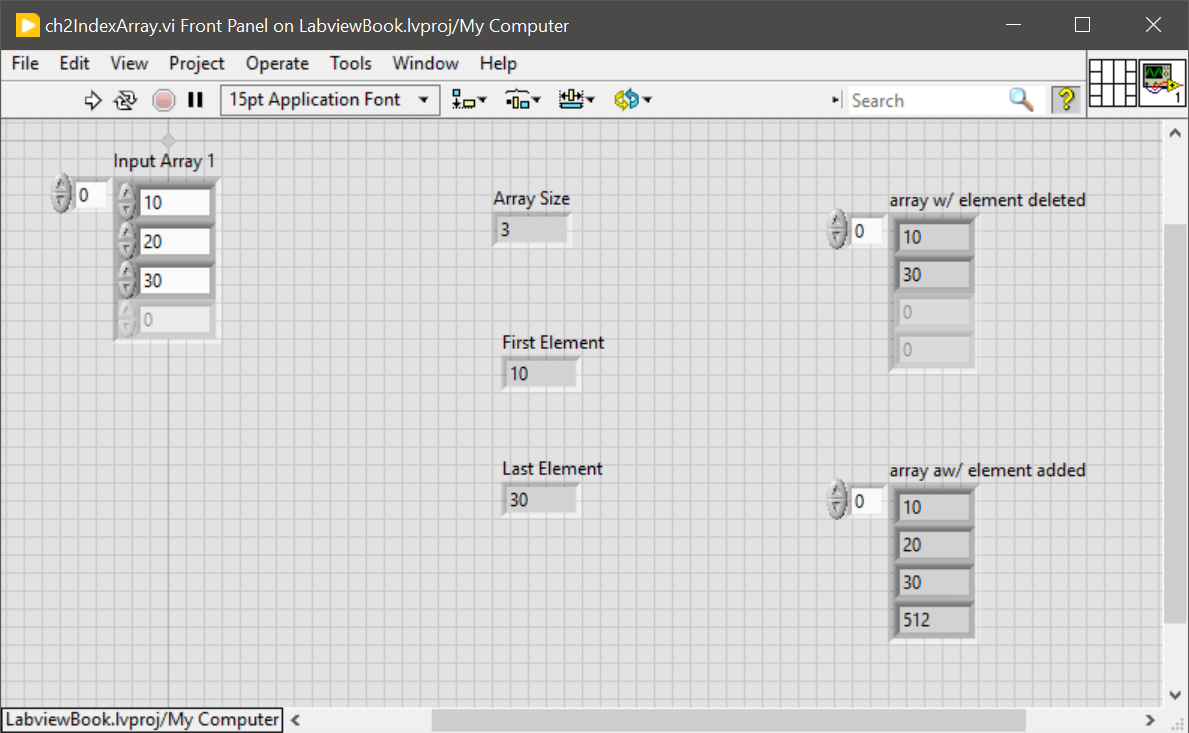
\includegraphics[width=\textwidth]{ch2IndexArrayFront}
	\caption{The results of fundamental operations on arrays.}
	\label{ch2IndexArrayFront}
\end{figure}

\subsubsection{Using arrays with loops}
In the previous section, we used loops to create a sequence of numbers. There was no way to store the numbers so the value was just printed to the screen on every loop.\\

Figure \ref{ch2eg6Block} shows a very simple way to extract a sequence from a loop. By branching the wire going into the shift register and connecting it to the while loop, $\labview$ creates what is known as an ``auto indexing tunnel''. The terminal has what looks like a blue \texttt{[]} inside of it. If yours is just a solid blue colour, \texttt{right click} on the terminal and select the indexing option. A solid blue box in this case means that the while loop will supply only the last value to that output.\\
\begin{figure}
	\centering
	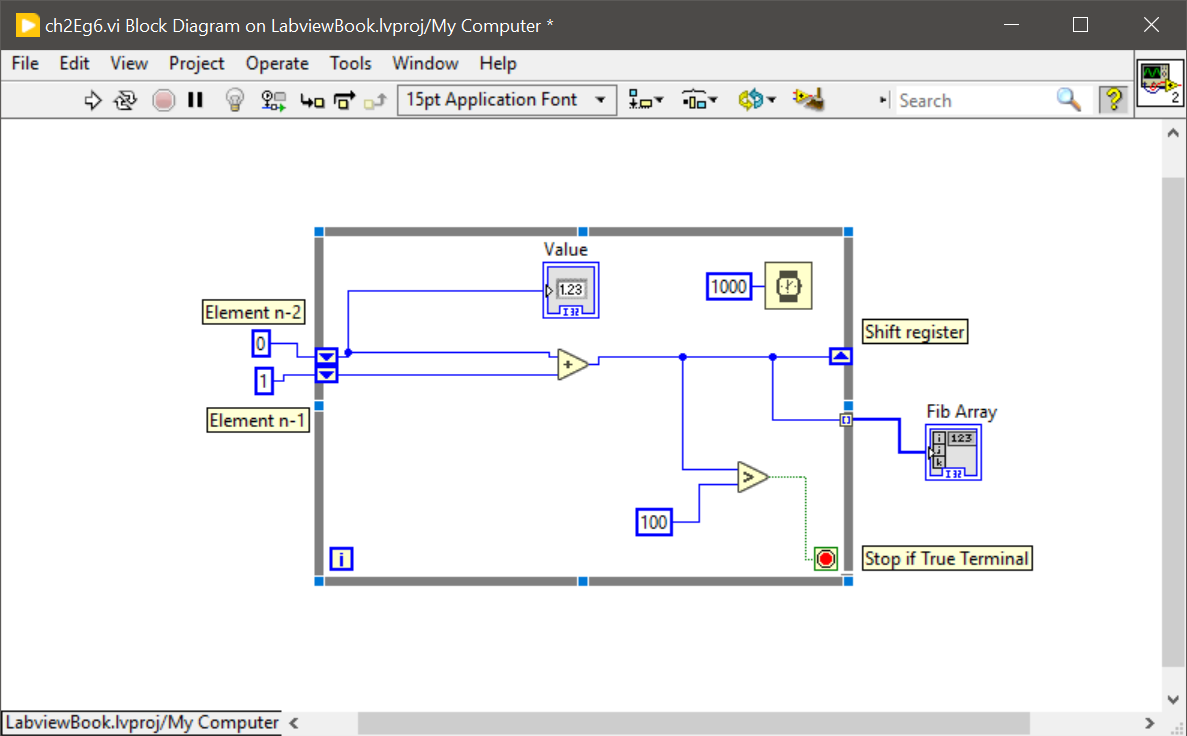
\includegraphics[width=\textwidth]{ch2eg6Block}
	\caption{Using auto indexing tunnels to create an array.}
	\label{ch2eg6Block}
\end{figure}
\begin{figure}
	\centering
	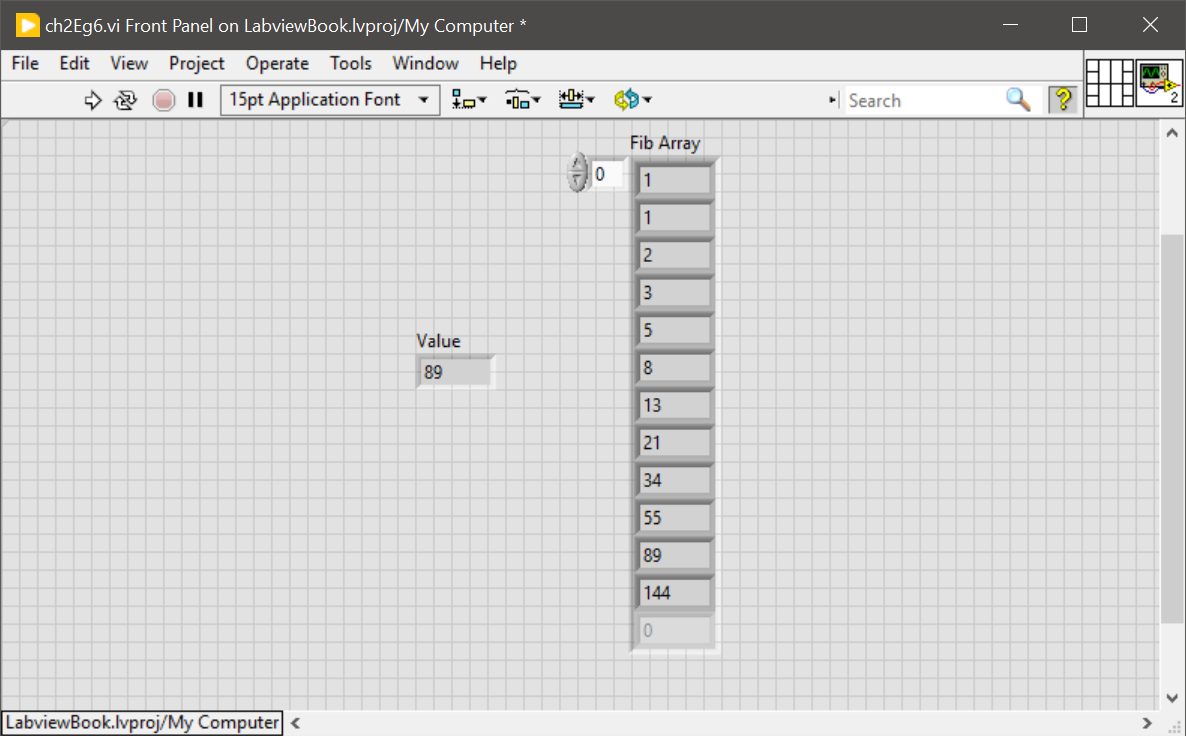
\includegraphics[width=\textwidth]{ch2eg6Front}
	\caption{The output of an auto indexing tunnel, do you notice what is wrong here?}
	\label{ch2eg6Front}
\end{figure}

Figure \ref{ch2eg6Front} shows the result of this computation, it is missing the first $0$ and there is another small mistake. We will fix both these mistakes in a moment.\\

Auto indexing of tunnels also work as inputs. Feeding an array into a for loop allows you to iterate over all its contents. In figure \ref{ch2SimpleForArray}, a previous example of element wise addition is recreated. The loop indexes input arrays, you may find the exact index by using the blue \texttt{i}, saving you the effort of manually indexing and inserting elements.\\
\begin{figure}
	\centering
	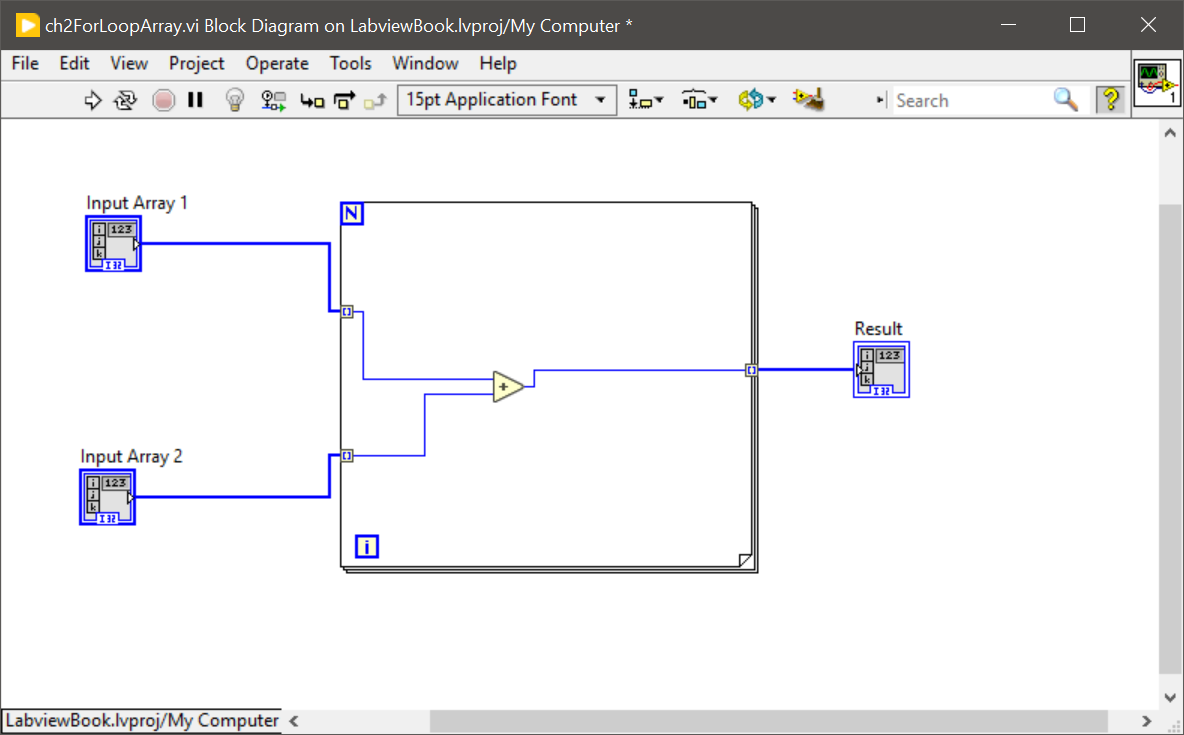
\includegraphics[width=\textwidth]{ch2SimpleForArray}
	\caption{Using auto indexing tunnels to create an array.}
	\label{ch2SimpleForArray}
\end{figure}

This tool becomes exceptionally powerful when combined with Arduino hardware, or any instrument really. Suppose you are controlling a LED, you can build a function that turns this LED on and off. You can then create an array with ones and zeros and feed it into a for loop. The for loop will pick off the elements one by one and send it to your LED function. If this sounds stupid to you, how did this document get to your computer screen, or into the printer if you are reading a hardcopy? The answer; bit by bit.\\

Let us now return to the Fibonacci sequence problem, in the previous example, the first $0$ was missing and the value $144$ is found hanging on the end of the array, this is larger than $100$, so it seems our condition value is ignored.\\

This occurs because, even though the value fed into our greater than function, the rest of the iteration executes. Thus the number $144$ comes along for a ride and is not cast into the depths of oblivion.\\

Figure \ref{ch2eg7} is, perhaps, an extravagant example on how to fix the two small mistakes in the previous example. There is a simpler fix which just requires the relocation of a single wire, can you find that fix?\\
\begin{figure}
	\centering
	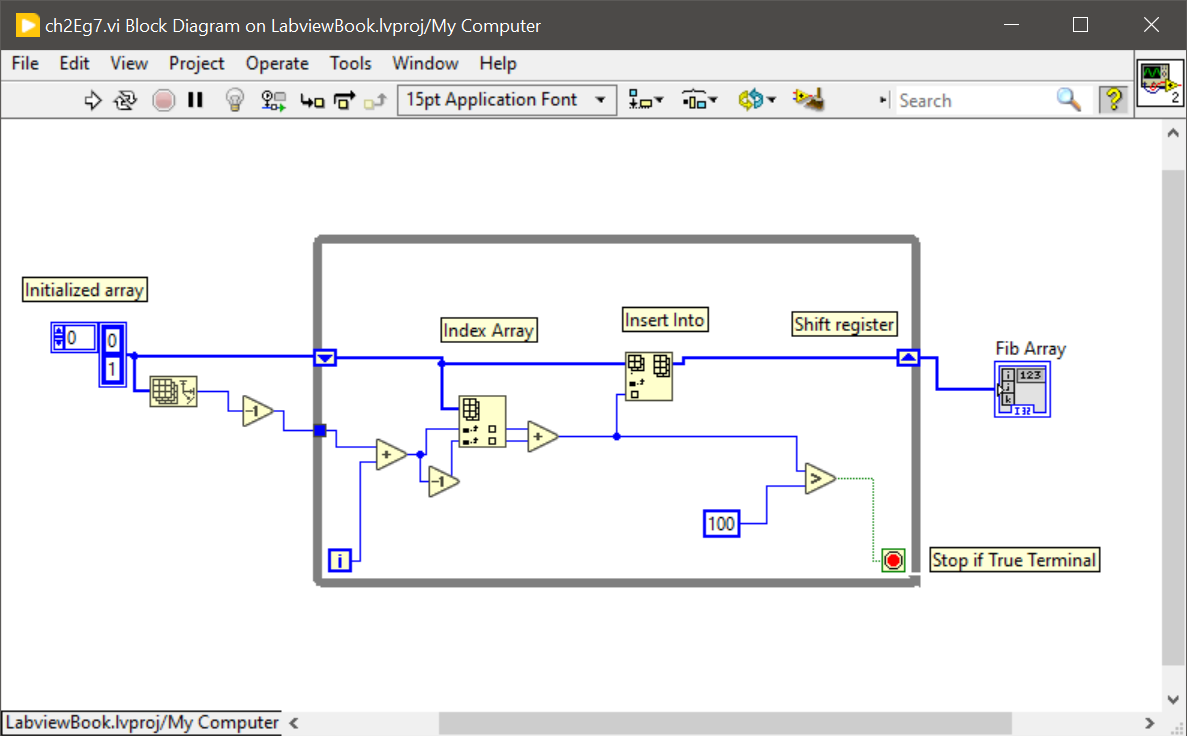
\includegraphics[width=\textwidth]{ch2eg7}
	\caption{A rewrite of the program that gives the expected results.}
	\label{ch2eg7}
\end{figure}

You should walk through the example in figure \ref{ch2eg7}, going step by step following the wires. Draw up this program on your own and see how it works. You can follow how $\labview$ executes this program by clicking on the light bulb in the top bar. This is the ``highlight execution'' button and is a useful tool to debug a program. If you grow tired of seeing the little signals passing through the wires, press the red button to stop the program.\\

\subsection{Clusters}
It is possible to group variables into bundles called clusters, this allows you to have one wire acting as a bus, caring around variables across your program. Figure \ref{ch2Cluster} shows how this is done using the ``Bundle'' function from the function palette.\\
\begin{figure}
	\centering
	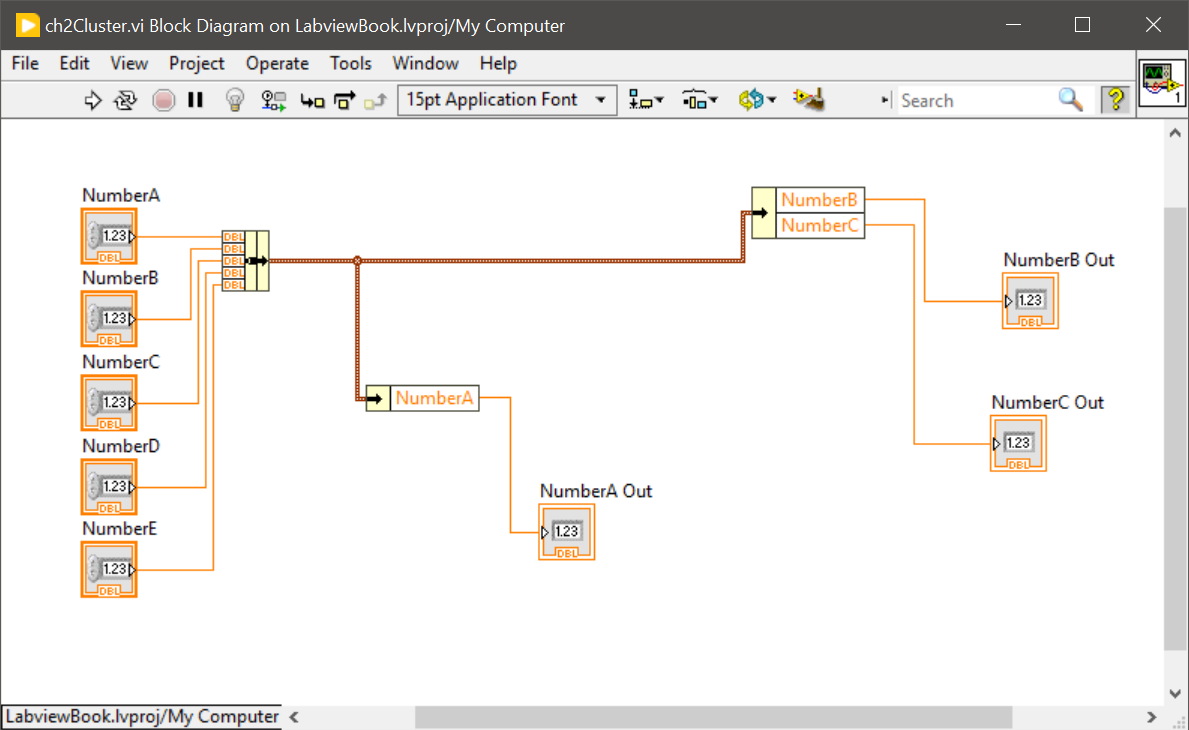
\includegraphics[width=\textwidth]{ch2Cluster}
	\caption{A group of numbers being bundled and unbundled.}
	\label{ch2Cluster}
\end{figure}

You can read an element from a cluster using either the ``Named Unbundle'' command or the ``Unbundle'' command. The named version uses the name of the wire being bundled, in this case the name is inherited from the control. This allows you to see at a glance what value you would like to choose. You can click and drag the blue terminals on the top or bottom of the bundle functions to increase or decrease the number of terminals. You can change the selected variables by clicking on their names and selecting a different one.\\

In the simple example, figure \ref{ch2Cluster}, you can see that it is possible to unbundle a variable at random, you do not need to unbundle everything at once. The name is slightly misleading however, when you unbundle a variable from a bus, you are not actually removing it, you are just making a copy of it. To change that variable, you have to either unbundle all the elements, change one, and wire everything back into a new bundle. This is tedious and error prone. A better way is to wire in an old bundle, into a ``Bundle'' function, and only selecting the variables you want to overwrite. The other values will stay unchanged.\\

This is all that you need for now when it comes to clusters. They are exceptionally useful for functions and keeping track of variables which are related to one another. There is also the topic of ``Type-definitions'' which properly exploits the utility of clusters. You can look forward to that in a later chapter.
\section{Creating functions}
You have no doubt seen so far how cluttered your block diagram can get. Figure \ref{ch2eg7} is a program that does one thing, generate an array of the Fibonacci numbers, how busy would the diagram get if we build upon this example? Very busy, so busy that you would wish you learned \texttt{C} instead.\\

You may clean up your code by grouping together functions in a little block, which is also known as a function. Before we get to that however, let us first take a detour into project management in $\labview$. Having a project groups your functions together and makes it easier to build upon your previous work.\\

\subsection{Project Management}
To create a project, on the startup screen, press the button that says ``Create Project'', see \ref{startup} on page \pageref{startup}. This will ask you what type of project you would like, there are quite a few templates to choose from, but for now just click on ``empty project''. A window will open up with your new empty untitled project like in figure \ref{newProjectPage}.\\
\begin{figure}
	\centering
	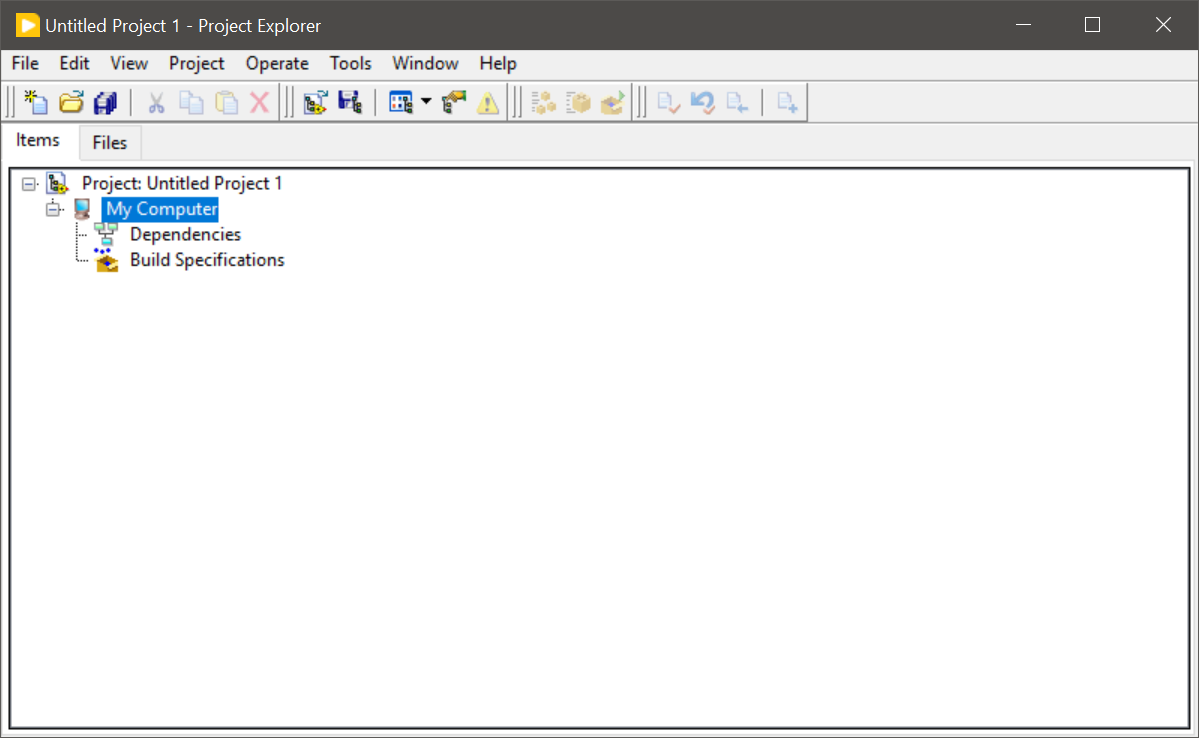
\includegraphics[width=\textwidth]{newProjectPage}
	\caption{A freshly baked project, it has nothing in it yet, you provide the rest.}
	\label{newProjectPage}
\end{figure}

From here you can create a new VI by going to ``File'' and pressing ``New...''. You can also create a virtual folder in the project by \texttt{right clicking} and pressing ``Create virtual folder''. This folder does not exist in your file system, instead it allows you to organise your project in meaningful sections. The examples in this book is also contained in a project, see figure \ref{BookProject}.\\
\begin{figure}
	\centering
	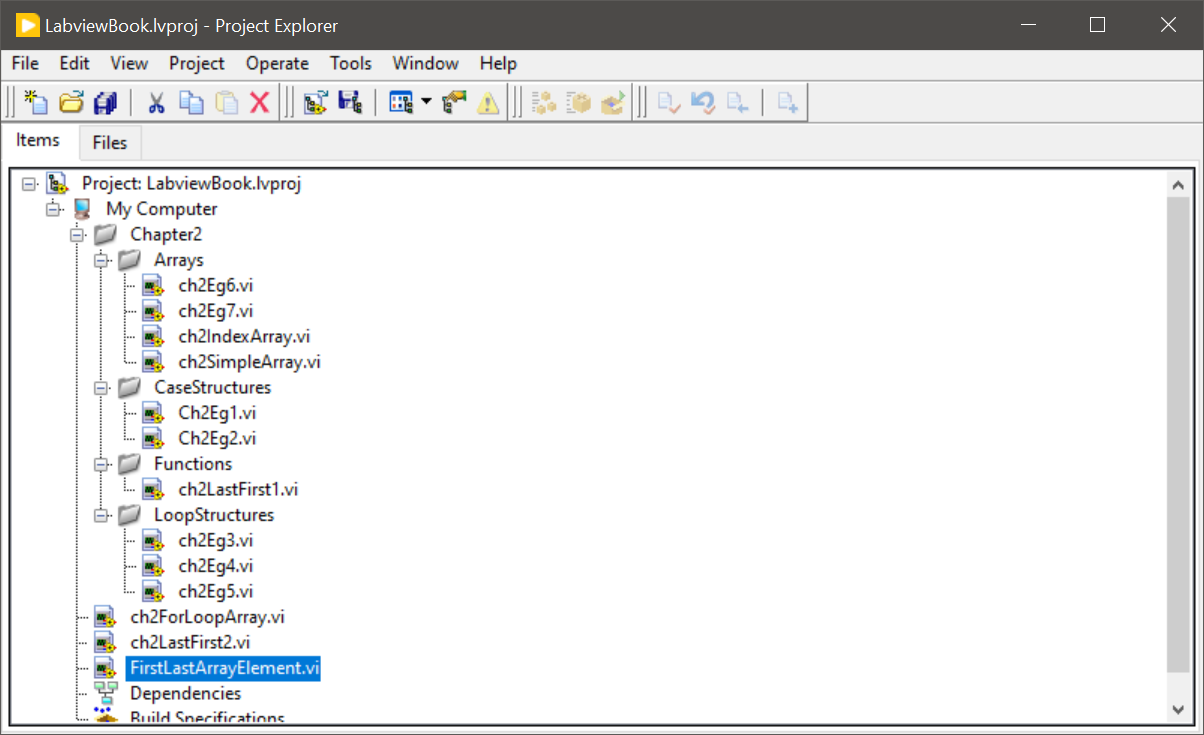
\includegraphics[width=\textwidth]{BookProject}
	\caption{The project used to keep track of all the examples in this book.}
	\label{BookProject}
\end{figure}

After you have created a VI in your project, it should open up by itself so you can start programming. You may also \texttt{double click} on a VI in the project manager to open up a particular VI. After you are done creating a program for launching ballistic missiles, you can save everything you are working on by going to file and then selecting ``Save All''. After that you can close the project manager and it will close all the other open VIs that are part of that particular project.\\

This is by no means a complete overview of the project manager, but it should be enough for you to get started. Once you have built some programs as functions, you can simply drag them into another VI to use them. We will get to that very soon.\\

\subsection{Creating a Function}
Just as a reminder, every block you have placed down in the block diagram is known as a function. For example, let us look at the ``Array Max \& Min'' function, in figure \ref{exampleMaxMinFunc}. I have wired in all the inputs and outputs to give you an idea of how it is used in an actual program. This is what we will be working toward.\\
\begin{figure}
	\centering
	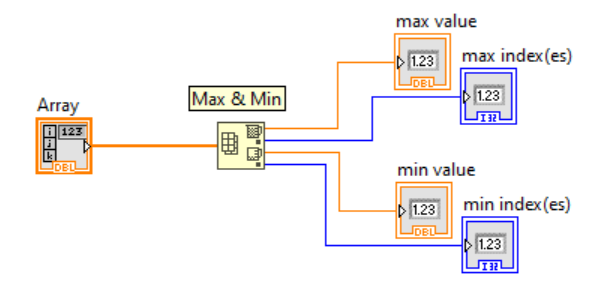
\includegraphics[width=0.75\textwidth]{exampleMaxMinFunc}
	\caption{The inputs and outputs of the Max \& Min function, we will use this as inspiration for our own function.}
	\label{exampleMaxMinFunc}
\end{figure}

Suppose we go back to figure \ref{ch2IndexArrayBlock}, on page \pageref{ch2IndexArrayBlock}, we extract the first and last element of an array by grabbing index $0$ and getting the last index by getting the array length and decrementing that by one. I have created a new VI to hold this program, seen in figure \ref{ch2LastFirst1}.\\
\begin{figure}
	\centering
	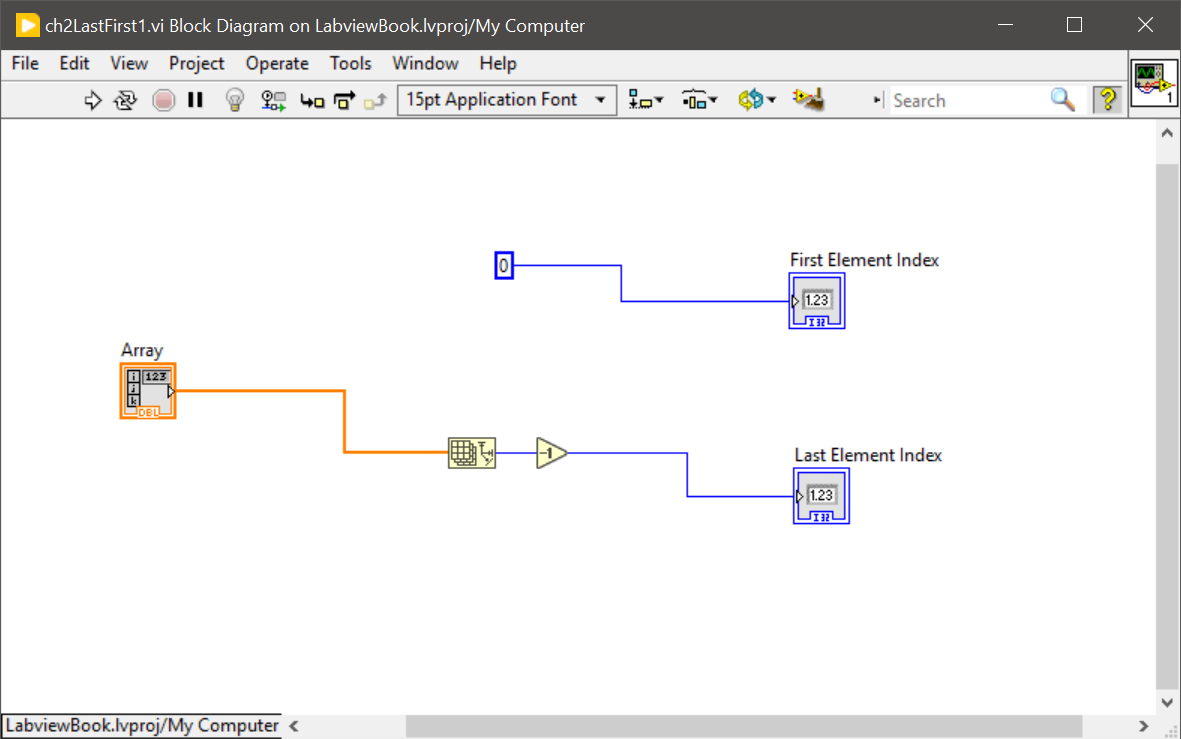
\includegraphics[width=\textwidth]{ch2LastFirst1}
	\caption{Prototype of a First and Last index function.}
	\label{ch2LastFirst1}
\end{figure}

We can now go one step further and use the index values to extract the two elements from an array. This makes sense because you either need the index values themselves or the actual values. You could create a program to do each function separately, but it does not hurt to do both. Figure \ref{ch2LastFirst2} shows how this is implemented. Note that every value not used is simply thrown away. If you are worried about program performance, just stop. Compiled $\labview$ programs are quite good at getting rid of parts of a program that is not used.\\

Now comes the fun part, drag a box and select the entire program excluding the control and indicator terminals, see figure \ref{ch2SelectionExample}. While still having the contents selected, from the taskbar go to ``Edit'' and select ``Create subVI from selection''. This wall squash everything into a little block, seen in figure \ref{ch2AutoSubVI}.\\
\begin{figure} %TODO Fix the condition figures to be the same size
	\centering
	\begin{subfigure}[b]{0.40\textwidth}
		\centering
		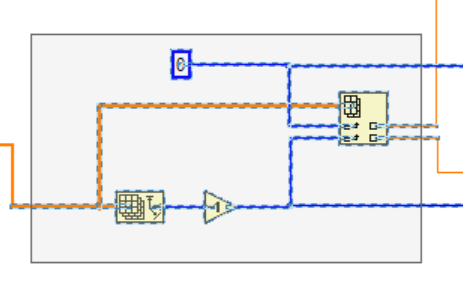
\includegraphics[width=\textwidth]{ch2SelectionExample}
		\caption{Everything in this box will go into our function.}
		\label{ch2SelectionExample}
	\end{subfigure}
	\hfil
	\begin{subfigure}[b]{0.40\textwidth}
		\centering
		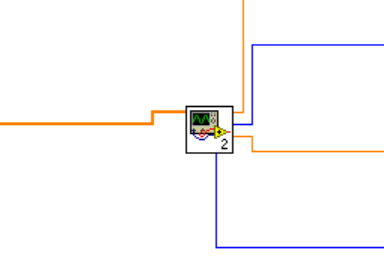
\includegraphics[width=\textwidth]{ch2SelectionSubVI}
		\caption{A newly created subVI, it is rather ugly.}
		\label{ch2SelectionSubVI}
	\end{subfigure}
	\caption{Creating a subVI, also known as a function.}
	\label{subVI}
\end{figure}

From a glance, it is not very clear what this function does, \texttt{double click} on this block to open up the VI. By a fluke, this example almost looks identical to the block diagram previously, bar the change in indicator names, see figure \ref{ch2AutoSubVI}. Rename these so that they make some sense.\\
\begin{figure}
	\centering
	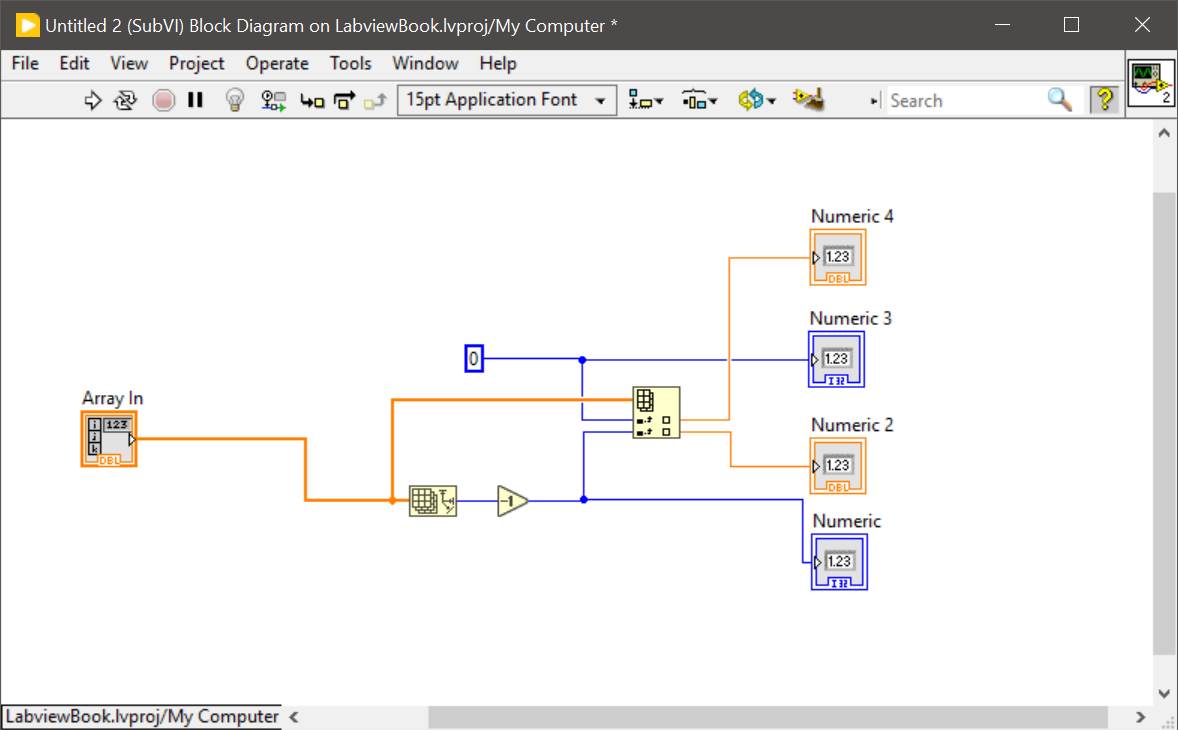
\includegraphics[width=\textwidth]{ch2AutoSubVI}
	\caption{The block diagram of the auto subVI function.}
	\label{ch2AutoSubVI}
\end{figure}

You can now double click on the icon in the top right corner of the window, figure \ref{ch2IconEdit} is the window that should open. This is the icon editor, it is like paint. Let your creative juices flow and create an icon that would make it clear what this function does among the hundreds of other functions in your programs. My attempt at an icon may be seen in figure \ref{ch2FuncMyIcon}.\\
\begin{figure}
	\centering
	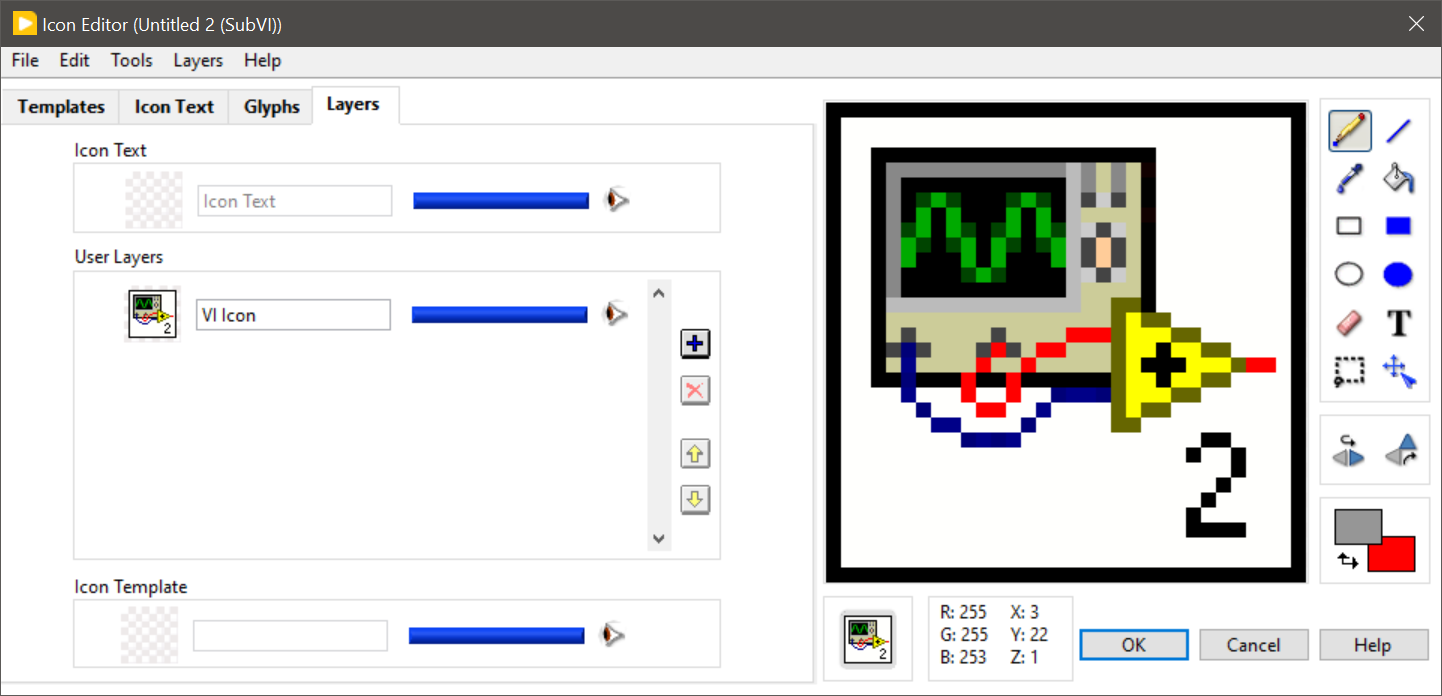
\includegraphics[width=\textwidth]{ch2IconEdit}
	\caption{The icon editor program.}
	\label{ch2IconEdit}
\end{figure}
\begin{figure}
	\centering
	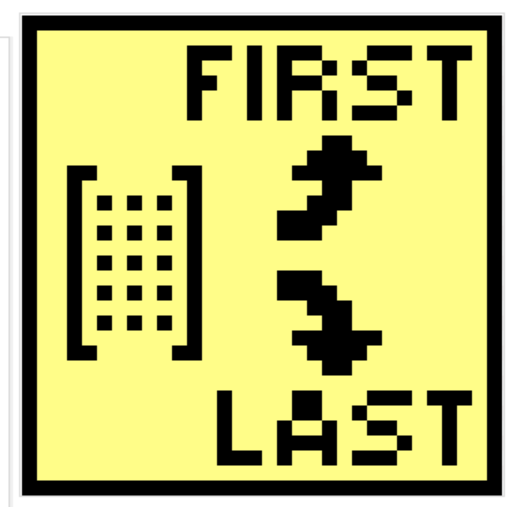
\includegraphics[width=0.25\textwidth]{ch2FuncMyIcon}
	\caption{This icon conveys more or less what the function does.}
	\label{ch2FuncMyIcon}
\end{figure}

With your new icon, you should focus on organising the wiring terminals. Figure \ref{ch2FuncPreGrid} shows how your terminal grid might look like. Note that this is only seen in the front panel window, not the block diagram window. If you \texttt{left click} on any of the colour filled terminals, you will see a blue box appear around the control that is associated with that terminal. The current layout might not make sense so let us redo it completely. \texttt{Right click} on the grid and select ``Disconnect All Terminals'' from the menu. You can then connect a control by clicking on an empty terminal (white) and clicking on a front panel element.
\begin{figure}
	\centering
	\begin{subfigure}[b]{0.40\textwidth}
		\centering
		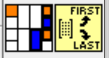
\includegraphics[width=\textwidth]{ch2FuncPreGrid}
		\caption{Automated creation of the terminal grid.}
		\label{ch2FuncPreGrid}
	\end{subfigure}
	\hfil
	\begin{subfigure}[b]{0.40\textwidth}
		\centering
		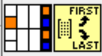
\includegraphics[width=\textwidth]{ch2FuncPostGrid}
		\caption{A manually wired input and output grid.}
		\label{ch2FuncPostGrid}
	\end{subfigure}
	\caption{The terminal grid for a function block.}
	\label{terminals}
\end{figure}

By convention we assume that inputs are on the left and outputs are on the right. Figure \ref{ch2FuncPostGrid} shows what might be a good layout, the orange square on the left is the array input while the alternating orange and blue indicators are the element and index outputs respectively. Here the first element comes from the top and the last element comes from the bottom, just like the icon would suggest. We now have our function ready for use, see figure \ref{exampleMyFunc}.\\
\begin{figure}
	\centering
	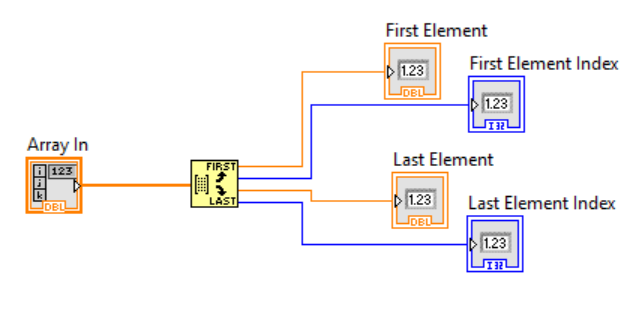
\includegraphics[width=0.75\textwidth]{exampleMyFunc}
	\caption{A fresh new function out of the oven, ready to be used in another program.}
	\label{exampleMyFunc}
\end{figure}

If you are wondering why we renamed the inputs and outputs to something useful, figure \ref{MyFuncContext}, is the context help message that appears when hovering over our function. The figure also shows a description of the function, this has to be supplied by you. You can do this by going to ``File'' in the taskbar and selecting ``VI Properties'', in this window, using the list-box named ``Category'' select the ``Documentation'' panel. Here you can write a little paragraph on your function.
\begin{figure}
	\centering
	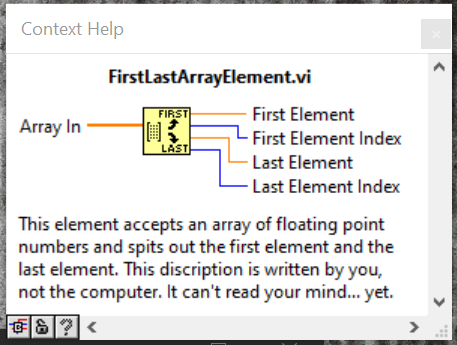
\includegraphics[width=0.50\textwidth]{MyFuncContext}
	\caption{The context help message for FirstLastArrayElement.vi.}
	\label{MyFuncContext}
\end{figure}

\subsection{Using a Function}
We are now ready to clean up the example in figure \ref{ch2IndexArrayBlock}, delete the part of the program that is being replaced with the function we just made. From the project manager window, click and drag the function over to the block diagram where you want the new function to live.\\

You can now wire in the function and you should have something that resembles figure \ref{ch2IndexArrayMyFunc}. That is it, I am sure you appreciate just how much neater the example looks.\\
\begin{figure}
	\centering
	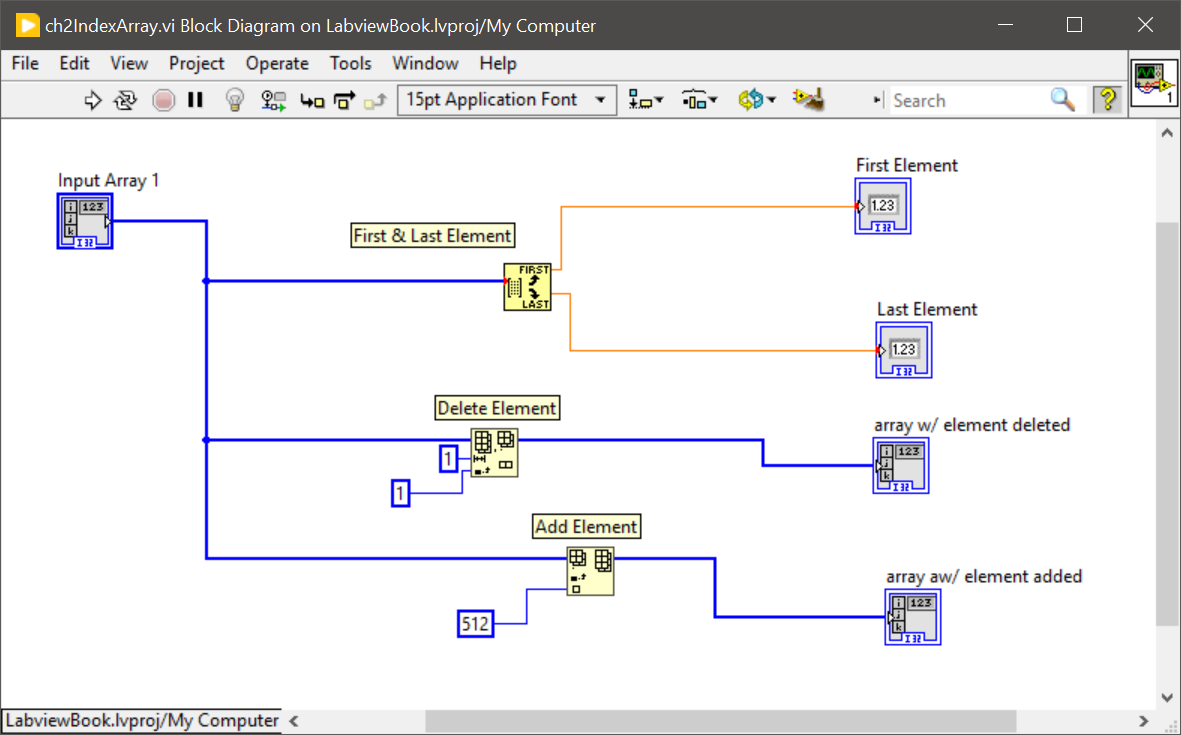
\includegraphics[width=\textwidth]{ch2IndexArrayMyFunc}
	\caption{A much neater example using a function we made ourselves.}
	\label{ch2IndexArrayMyFunc}
\end{figure}

This function has a problem, it does not know what type of array is piped into it. The built in functions found in $\labview$ adapt to their inputs. They are what is known as ``malleable'' VIs. This topic is not really advanced, it is easy to create a malleable VI yourself. The difficulty is dealing with typecasting and how $\labview$ deals with types internally. This will be covered in a future chapter.
 \newpage
\section{Slightly more advanced Mini Projects}
\begin{enumerate}
	\item Build a simple 4-function calculator, that is, a program which takes two inputs and performs either addition, subtraction, multiplication or division.\\
	
	You have also seen how element wise operations are preformed on arrays, write a separate program that takes an array as an input and then gives the user the ability to choose a single index on which the operation is performed or if the users uses index $-1$, the operation is performed on the entire array.\\
	
	Search the $\labview$ helpfiles for the topic known as an ``polymorphic VI'', this type of VI allows you to stack different operations into a single function. Try to merge the two programs you have created into a function which allows the user to choose between two single value inputs, and an array input with index and single value inputs.
	
	\item There is a very handy little function called ``String to Byte Array'', to find it, open the function palette and in the top right corner you will see the ``search'' box, use this feature to find anything you struggle to find in the conventional means. This particular function takes a string type as an input and converts it into an array of 8-bit unsigned integers according to ASCII encoding.\\
	
	Read up on ``Caesar's cypher'', use the above function to create a program that encrypts a block of text. Also create a program that decrypts a block of text. For both you will need a method to select the shift number. Send this encrypted block of text to your friends, along with the shift number, so that they can read your secret message.\\
	
	Request an encrypted message from your friends without a shift number. Write a program that can crack this cypher, this should be simple since the cypher is very easy to crack, any encrypted text can be deciphered by a maximum of 255 shifts since the block should be pure ASCII.
	
	\item For the previous project you used the ``String to Byte Array'', this time, use the ``Number To Boolean Array'' to write a function which converts the input from the ``String to Byte Array'' to patterns of light. This means you require a program with eight indicator lights, representing an 8-bit register, and then the program should be able to use those two functions to convert a string of characters into patterns of light. This will be used in the next chapter to create advanced programs for the Arduino.\\
	
	If this is proving to be difficult, if it is trivially easy for you then you should look for a more advanced book on $\labview$, write a program that converts a string into an array of bytes, wire this array of bytes into a for loop. Inside the for loop, use the number to boolean array function, wire this array into another for loop. Inside of this nested for loop, use a timer function to wait for a 100ms, the value coming from the boolean array can be piped into an LED. This will give you an idea how a TV remote works.
\end{enumerate}